\documentclass{beamer}

\usepackage[spanish]{babel}
\usepackage[utf8]{inputenc}
\usepackage{cite}
\usepackage{amsmath,amssymb,amsfonts}
\usepackage{algorithmic}
\usepackage{graphicx}
\usepackage{textcomp}
\usepackage{xcolor}
\usepackage{fancyhdr}
\usepackage{listings}
\usepackage{float}
\usepackage{blindtext}
\usepackage{newtxmath}
\usepackage{wrapfig}
\usepackage{mathtools}
\usepackage{breqn}
\usepackage{titlesec}
\usepackage{multirow}

\usepackage[flushleft]{threeparttable}
\usepackage{makecell,booktabs}

\usepackage[hyphens]{url}
\usepackage[hidelinks]{hyperref}


\lstdefinestyle{code}{%
backgroundcolor=\color{gray!1},
basicstyle=\ttfamily\small,
commentstyle=\color{green!60!black},
keywordstyle=\color{magenta},
stringstyle=\color{blue!50!red},
showstringspaces=false,
%captionpos=b,
numbers=left,
numberstyle=\footnotesize\color{gray},
numbersep=5pt,
%stepnumber=2,
tabsize=2,
%frame=L,
%framerule=1pt,
%rulecolor=\color{red},
breaklines=true,
}
\decimalpoint 
\usefonttheme[onlymath]{serif}
\setlength{\columnsep}{0.3mm}
\usetheme{Frankfurt}

\author[Visión por Computadora]{Madrigal-Custodio Jesús A., Tevera-Ruiz Alejandro, Torres-Martínez Luis Á.}
\title{Súper-resolución de imágenes}
\subtitle{Comparativa de métodos}
\institute[CINVESTAV]{Maestría en Ciencias en Robótica y Manufactura Avanzada}
\date{12 de abril de 2022}

% defs
\def\cmd#1{\texttt{\color{red}\footnotesize $\backslash$#1}}
\def\env#1{\texttt{\color{blue}\footnotesize #1}}
\definecolor{deepblue}{rgb}{0,0,0.5}
\definecolor{deepred}{rgb}{0.6,0,0}
\definecolor{deepgreen}{rgb}{0,0.5,0}
\definecolor{halfgray}{gray}{0.55}

\lstset{
    basicstyle=\ttfamily\small,
    keywordstyle=\bfseries\color{deepblue},
    emphstyle=\ttfamily\color{deepred}, 
    stringstyle=\color{deepgreen},
    numbers=left,
    numberstyle=\small\color{halfgray},
    rulesepcolor=\color{red!20!green!20!blue!20},
    frame=shadowbox,
}

% Extras
\numberwithin{equation}{section}
\numberwithin{figure}{section}
\numberwithin{table}{section}
\graphicspath{ {./Imagenes/} }
% Control de tamaño de imágenes por variable
\newcommand{\scaleFigures}{0.7}

\graphicspath{ {Imagenes/} }

\justifying

\begin{document}

\renewcommand{\tablename}{Tabla}

\begin{frame}
    \titlepage
    \begin{figure}[h]
        \begin{center}
            
\includegraphics[width=0.1\linewidth]{Cinvestav.jpg}
        \end{center}
    \end{figure}
\end{frame}

\begin{frame}
    \tableofcontents[sectionstyle=show,subsectionstyle=show/shaded/hide,subsubsectionstyle=show/shaded/hide]
\end{frame}


\section{Introducción}
    \begin{frame}
    \frametitle{Objetivos del proyecto}
    Introducción, salu2
    \begin{block}{Objetivos}
        \begin{enumerate}
            \item Desarrollar 
        \end{enumerate}
    \end{block}

\end{frame}

\begin{frame}
    \frametitle{Objetivos del proyecto}
    \begin{block}{Objetivos}
     
    \end{block}

\end{frame}

\section{Antecedentes}
    \begin{frame}{Súper Resolución}
    Bajo un enfoque \emph{clásico}, existen tres formas de mejorar la resolución 
    de una imagen:


    \begin{block}{Métodos}
        \begin{itemize}
            \item Amplificación de detalles existentes
            \item Suma de múltiples frames
            \item Único frame
        \end{itemize}
    \end{block}

\end{frame}

\begin{frame}{Predicción de resolución a partir de un único frame}
    ¿Cómo aumentar la densidad de pixeles de una imagen? 

    \pause
    \vspace{0.5cm}
    
    Predicción, aproximación... 
    
    \pause 

    \vspace{0.5cm}

    \begin{block}{Tipos}
        Dentro de las propuestas se encuentran los interpoladores:
        \begin{itemize}
            \item \emph{Adaptativos}: Algoritmos cambiantes por pixel
            \item \emph{No adaptativos}: Algoritmos estáticos a través de Algoritmos
            adyacentes. 
        \end{itemize}
    \end{block}

    Algunos de ellos incluyen algoritmos como \emph{vecino más cercano, bilineal, bicúbica,
    spline, entre otros.}
    
\end{frame}

\begin{frame}{Interpoladores no adaptativos}
    
    \begin{block}{Tipos}
        \begin{itemize}
            \item \textbf{Vecino más cercano} - Vecindad 1x1
            \item \textbf{Bilineal} - Vecindad 2x2 con promedios ponderados
            \item \textbf{Bicúbica} - Vecindad 4x4 con promedios ponderados 
        \end{itemize}
    \end{block}


    
    \begin{figure}[H]
        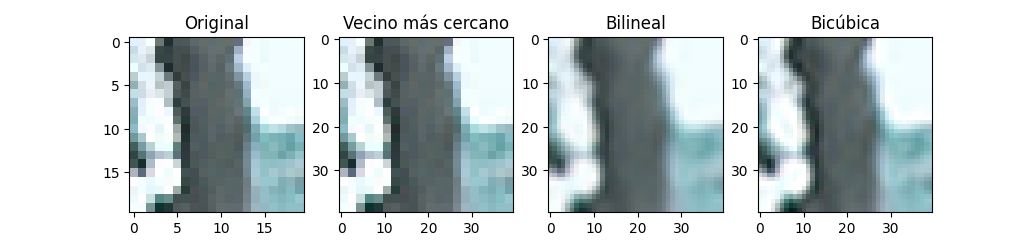
\includegraphics[scale = 0.45 ]{ tipos_interpoladores.png }
        \centering
        \caption{ Algoritmos de interpolación no adaptativos }
        \label{fig:interpoladores}
    \end{figure}

\end{frame}

\begin{frame}{Efectos de la interpolación}
    
    Todos los interpoladores no adaptativos intentan encontrar un equilibrio óptimo
    entre tres efectos no deseados: halos de borde, desenfoque y \emph{aliasing}. En la 
    Figura \ref{fig:efectos_inter} puede observarse el efecto para cada caso. 
    
    \begin{figure}[H]
        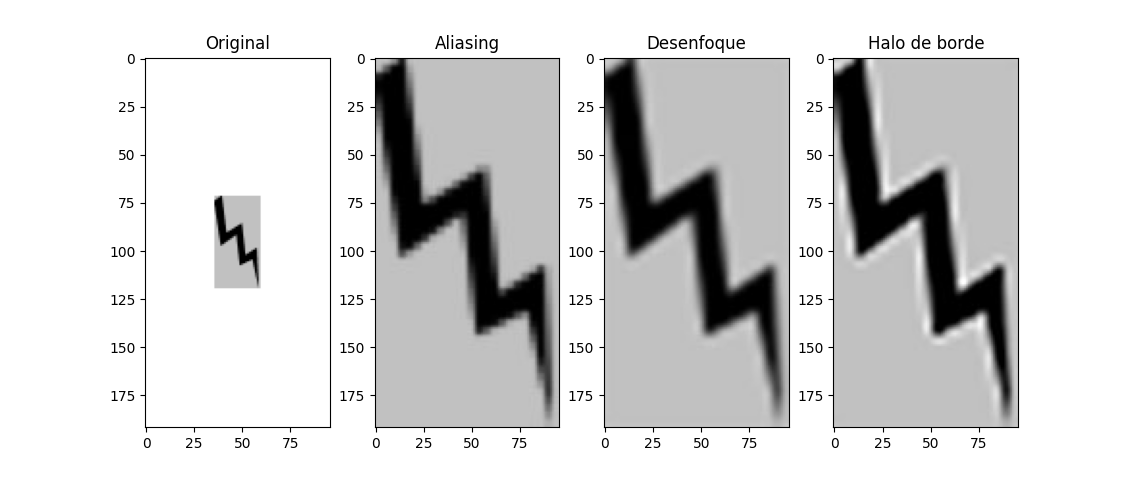
\includegraphics[scale = 0.35 ]{ efectos_inter.png }
        \centering
        \caption{ Efectos de interpolación}
        \label{fig:efectos_inter}
    \end{figure}

\end{frame}


\begin{frame}{Mejorar la interpolación de imágenes}
    
    \begin{block}{Dentro de las propuestas, \emph{Freeman et al} propone:}
        \begin{enumerate}
            \item La relación entre parches de alta y baja resolución
            es independiente del contraste de la imagen. 
            \item Los detalles están en las altas frecuencias 
        \end{enumerate}
    \end{block}

    \begin{figure}[H]
        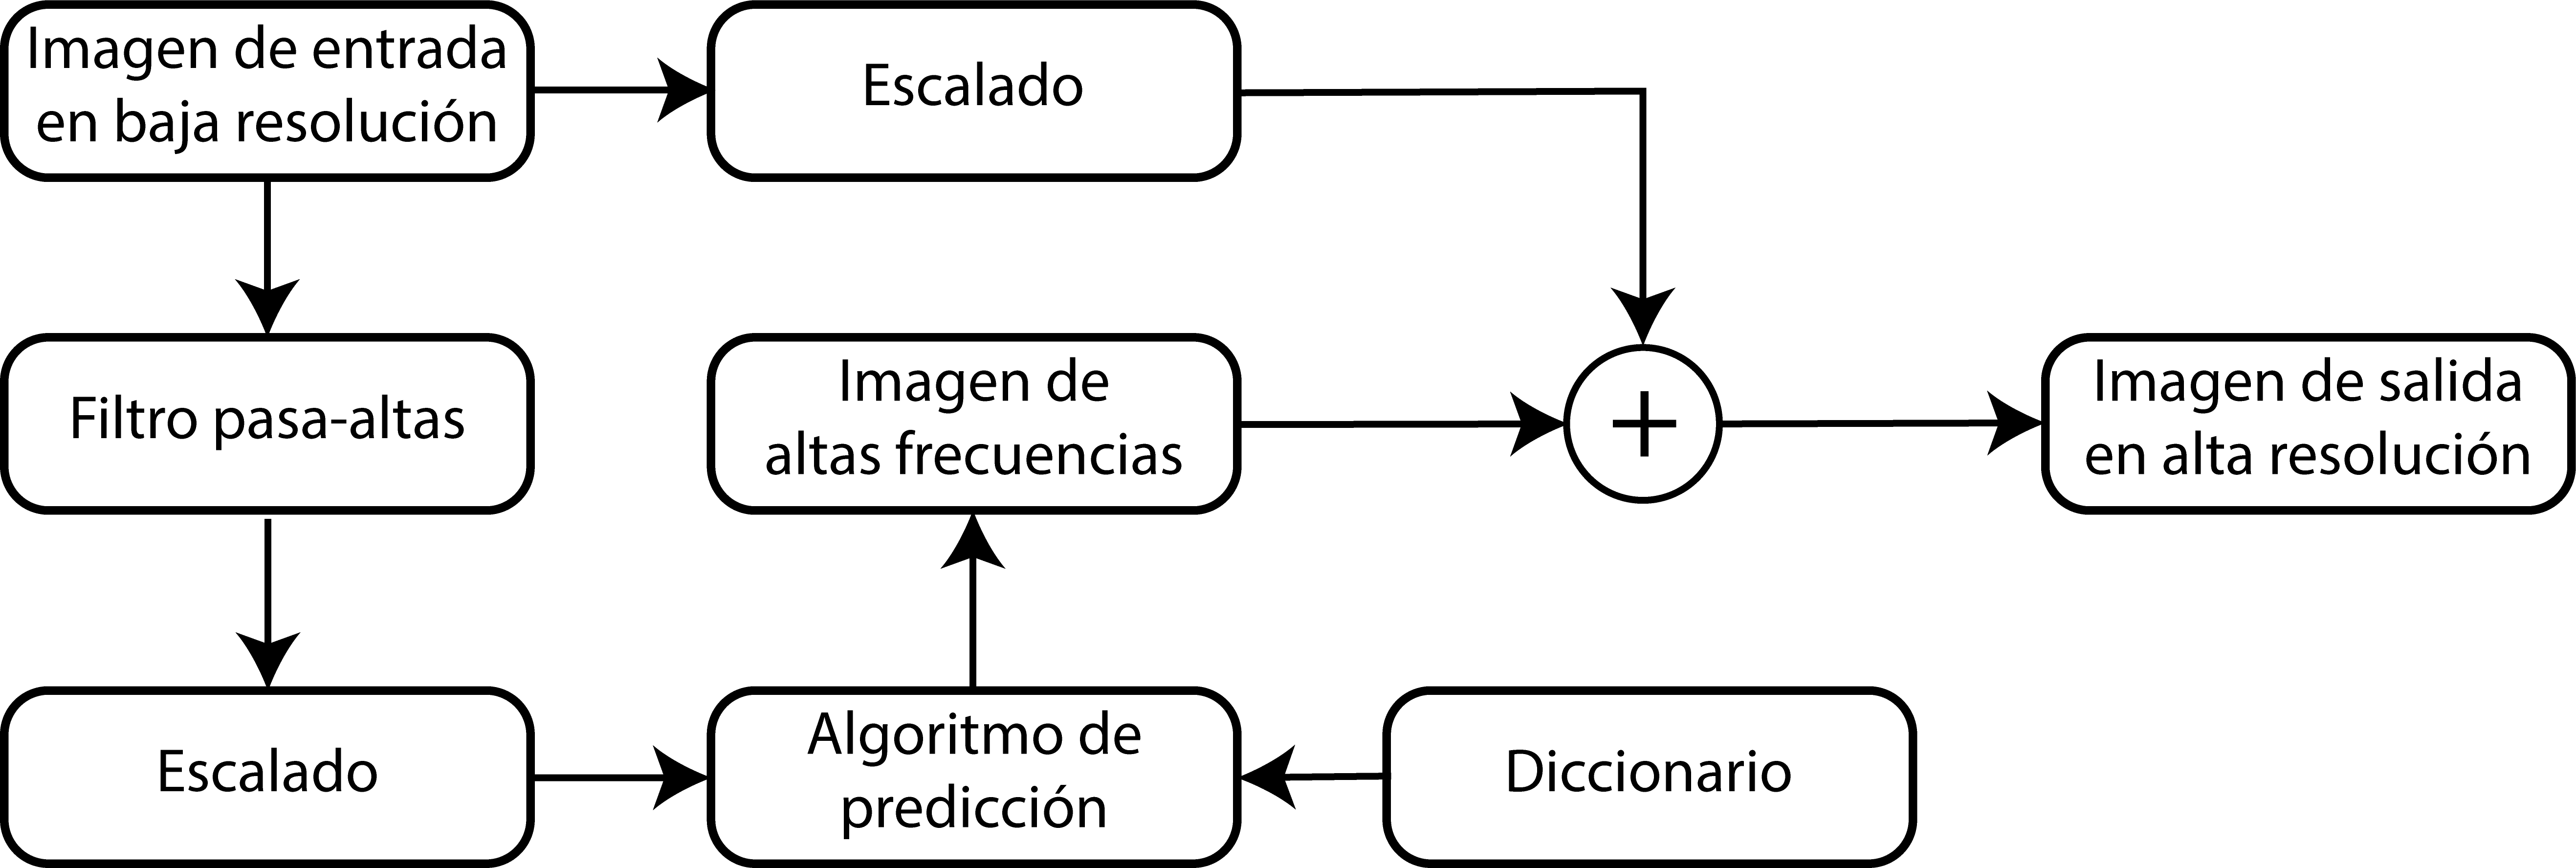
\includegraphics[scale = 0.4]{ fr_algoritmo.png }
        \centering
        \caption{ Algoritmo de súper resolución }
        \label{fig:fr_algoritmo}
    \end{figure}
    
\end{frame}

\begin{frame}{Diccionario}

    \begin{figure}[H]
        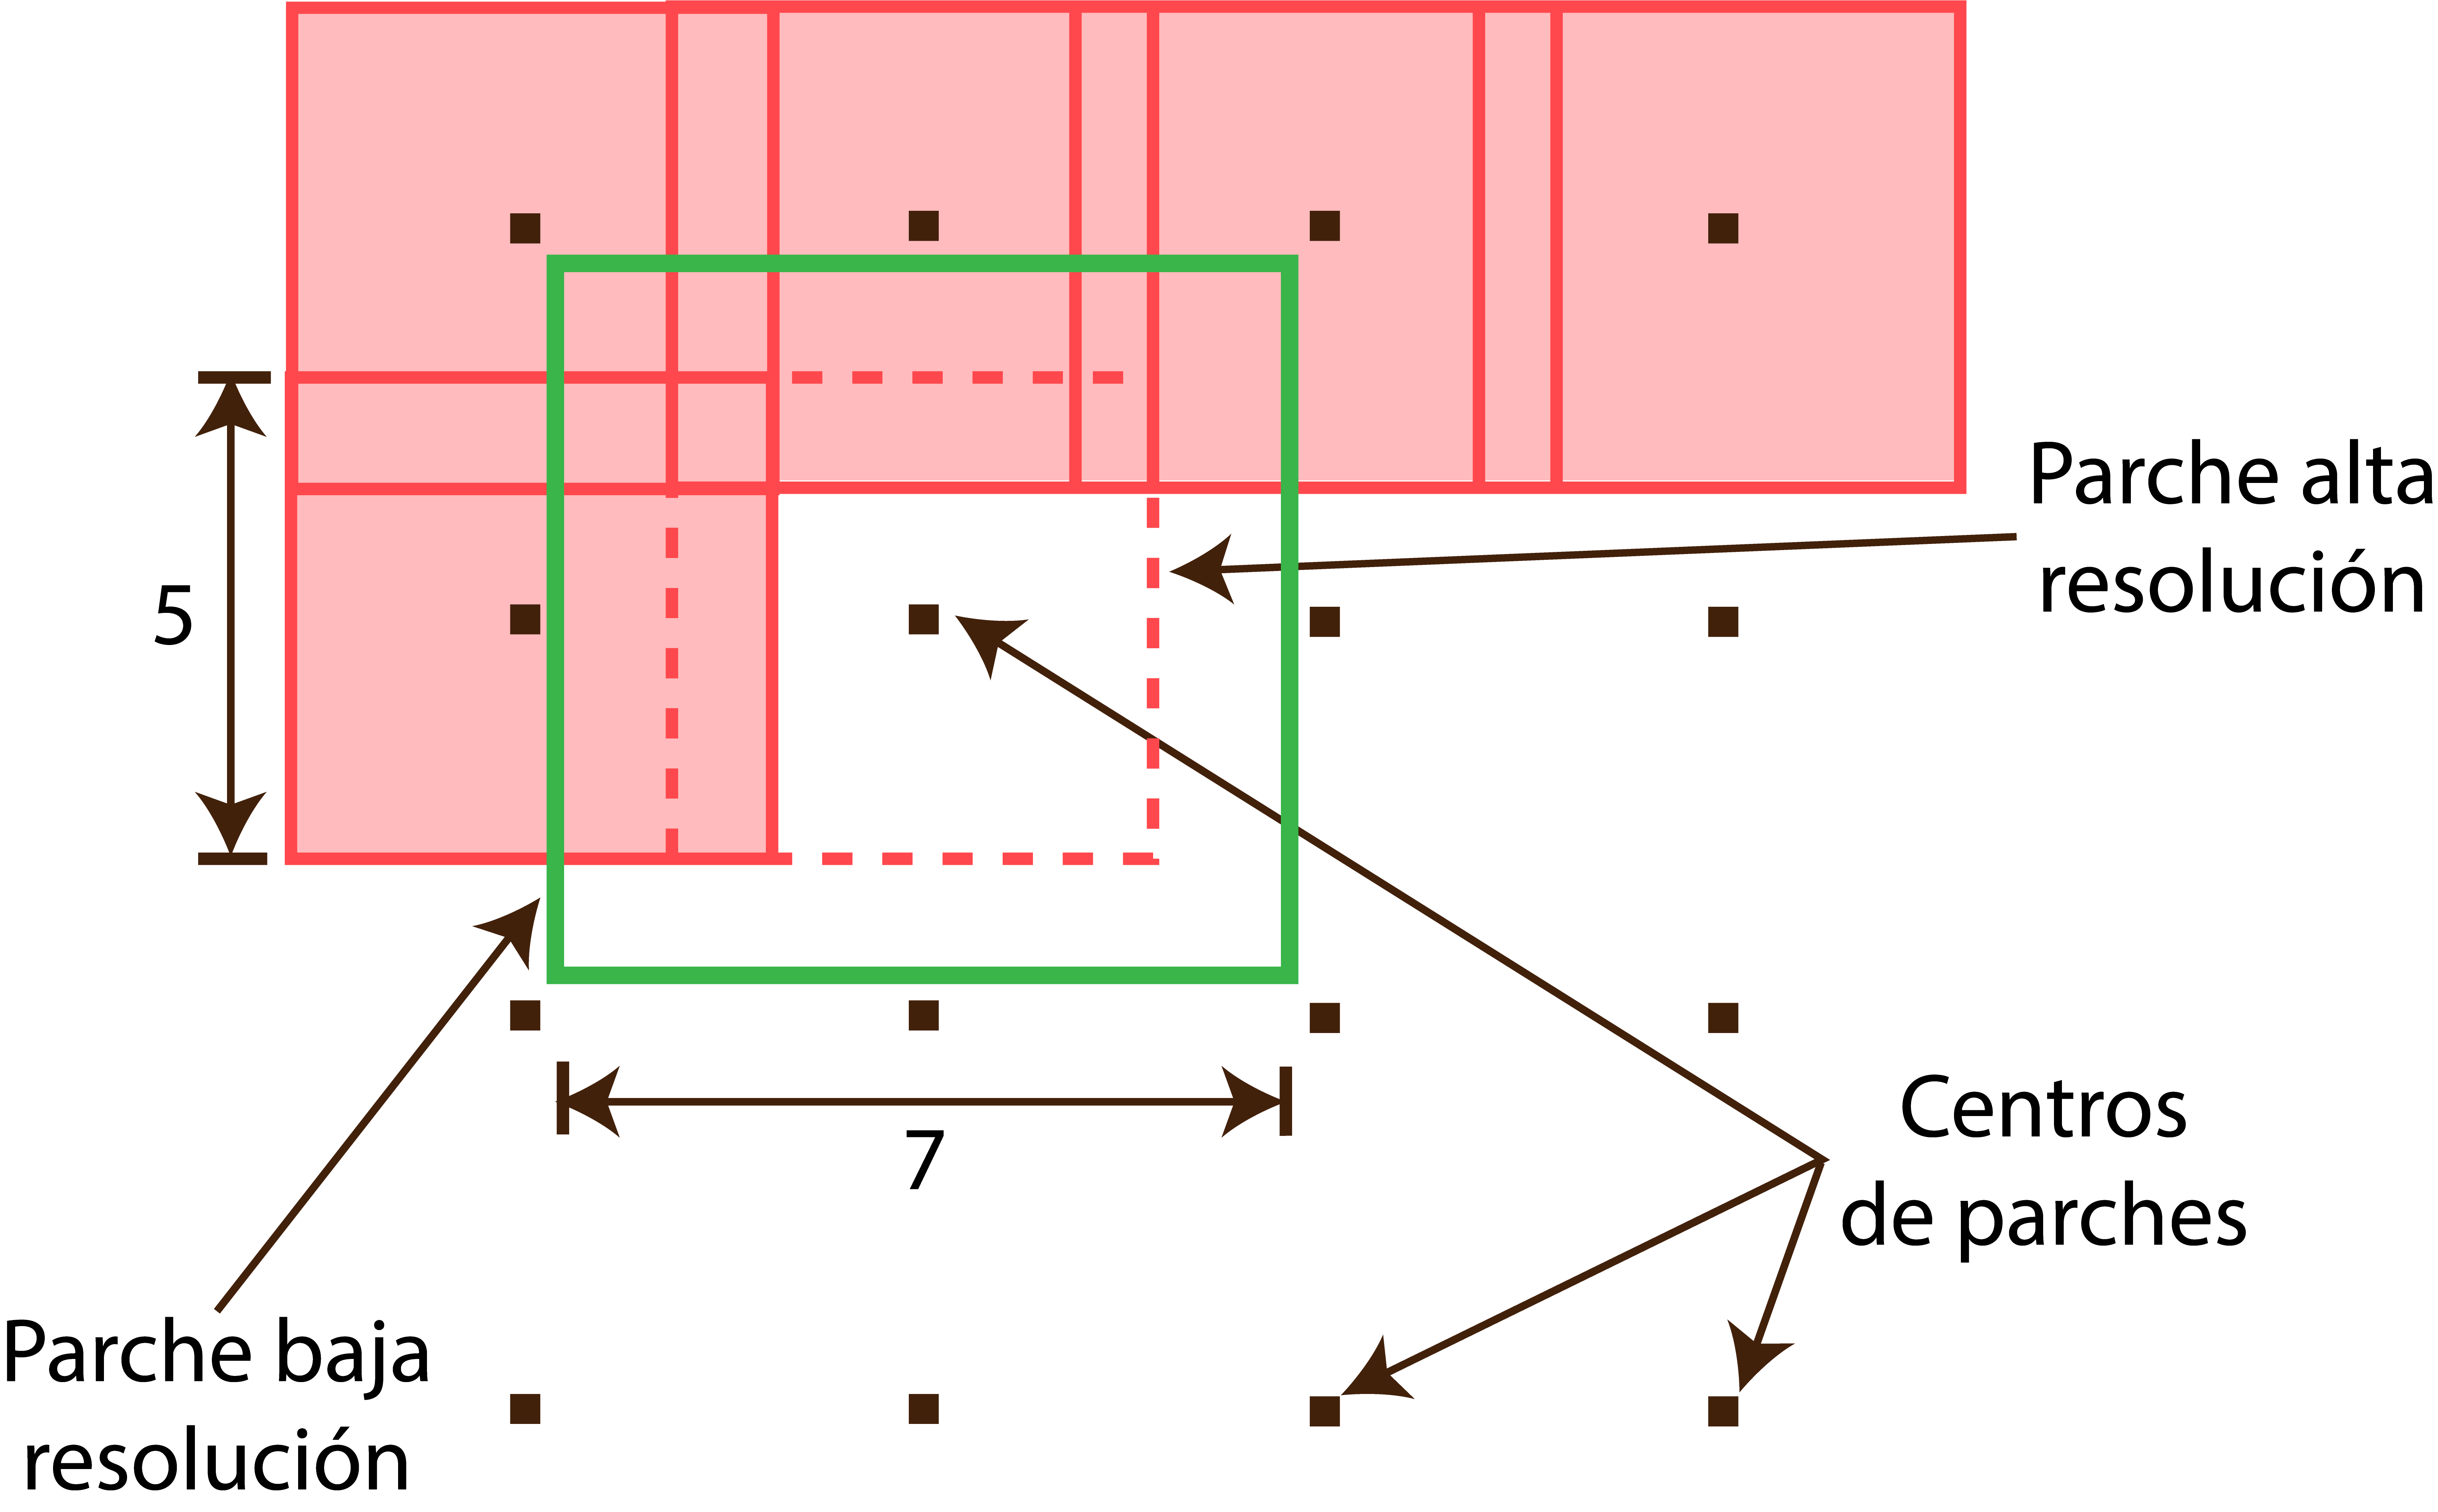
\includegraphics[scale = 0.18]{ fr_diccionario.png }
        \centering
        \caption{ Adquisición de parches de cada imagen}
        \label{fig:fr_dic}
    \end{figure}

    En específico, los parches de baja resolución deben reordenarse como un vector 
    en $\mathbb{R}^{1\times49}$ concatenado con la primera fila y primera columna
    del parche de alta resolución, resultando en un \textbf{vector para búsqueda} en $\mathbb{R}^{1\times59}$.
    
\end{frame}


\begin{frame}{Algoritmo de predicción}

    \begin{figure}[H]
        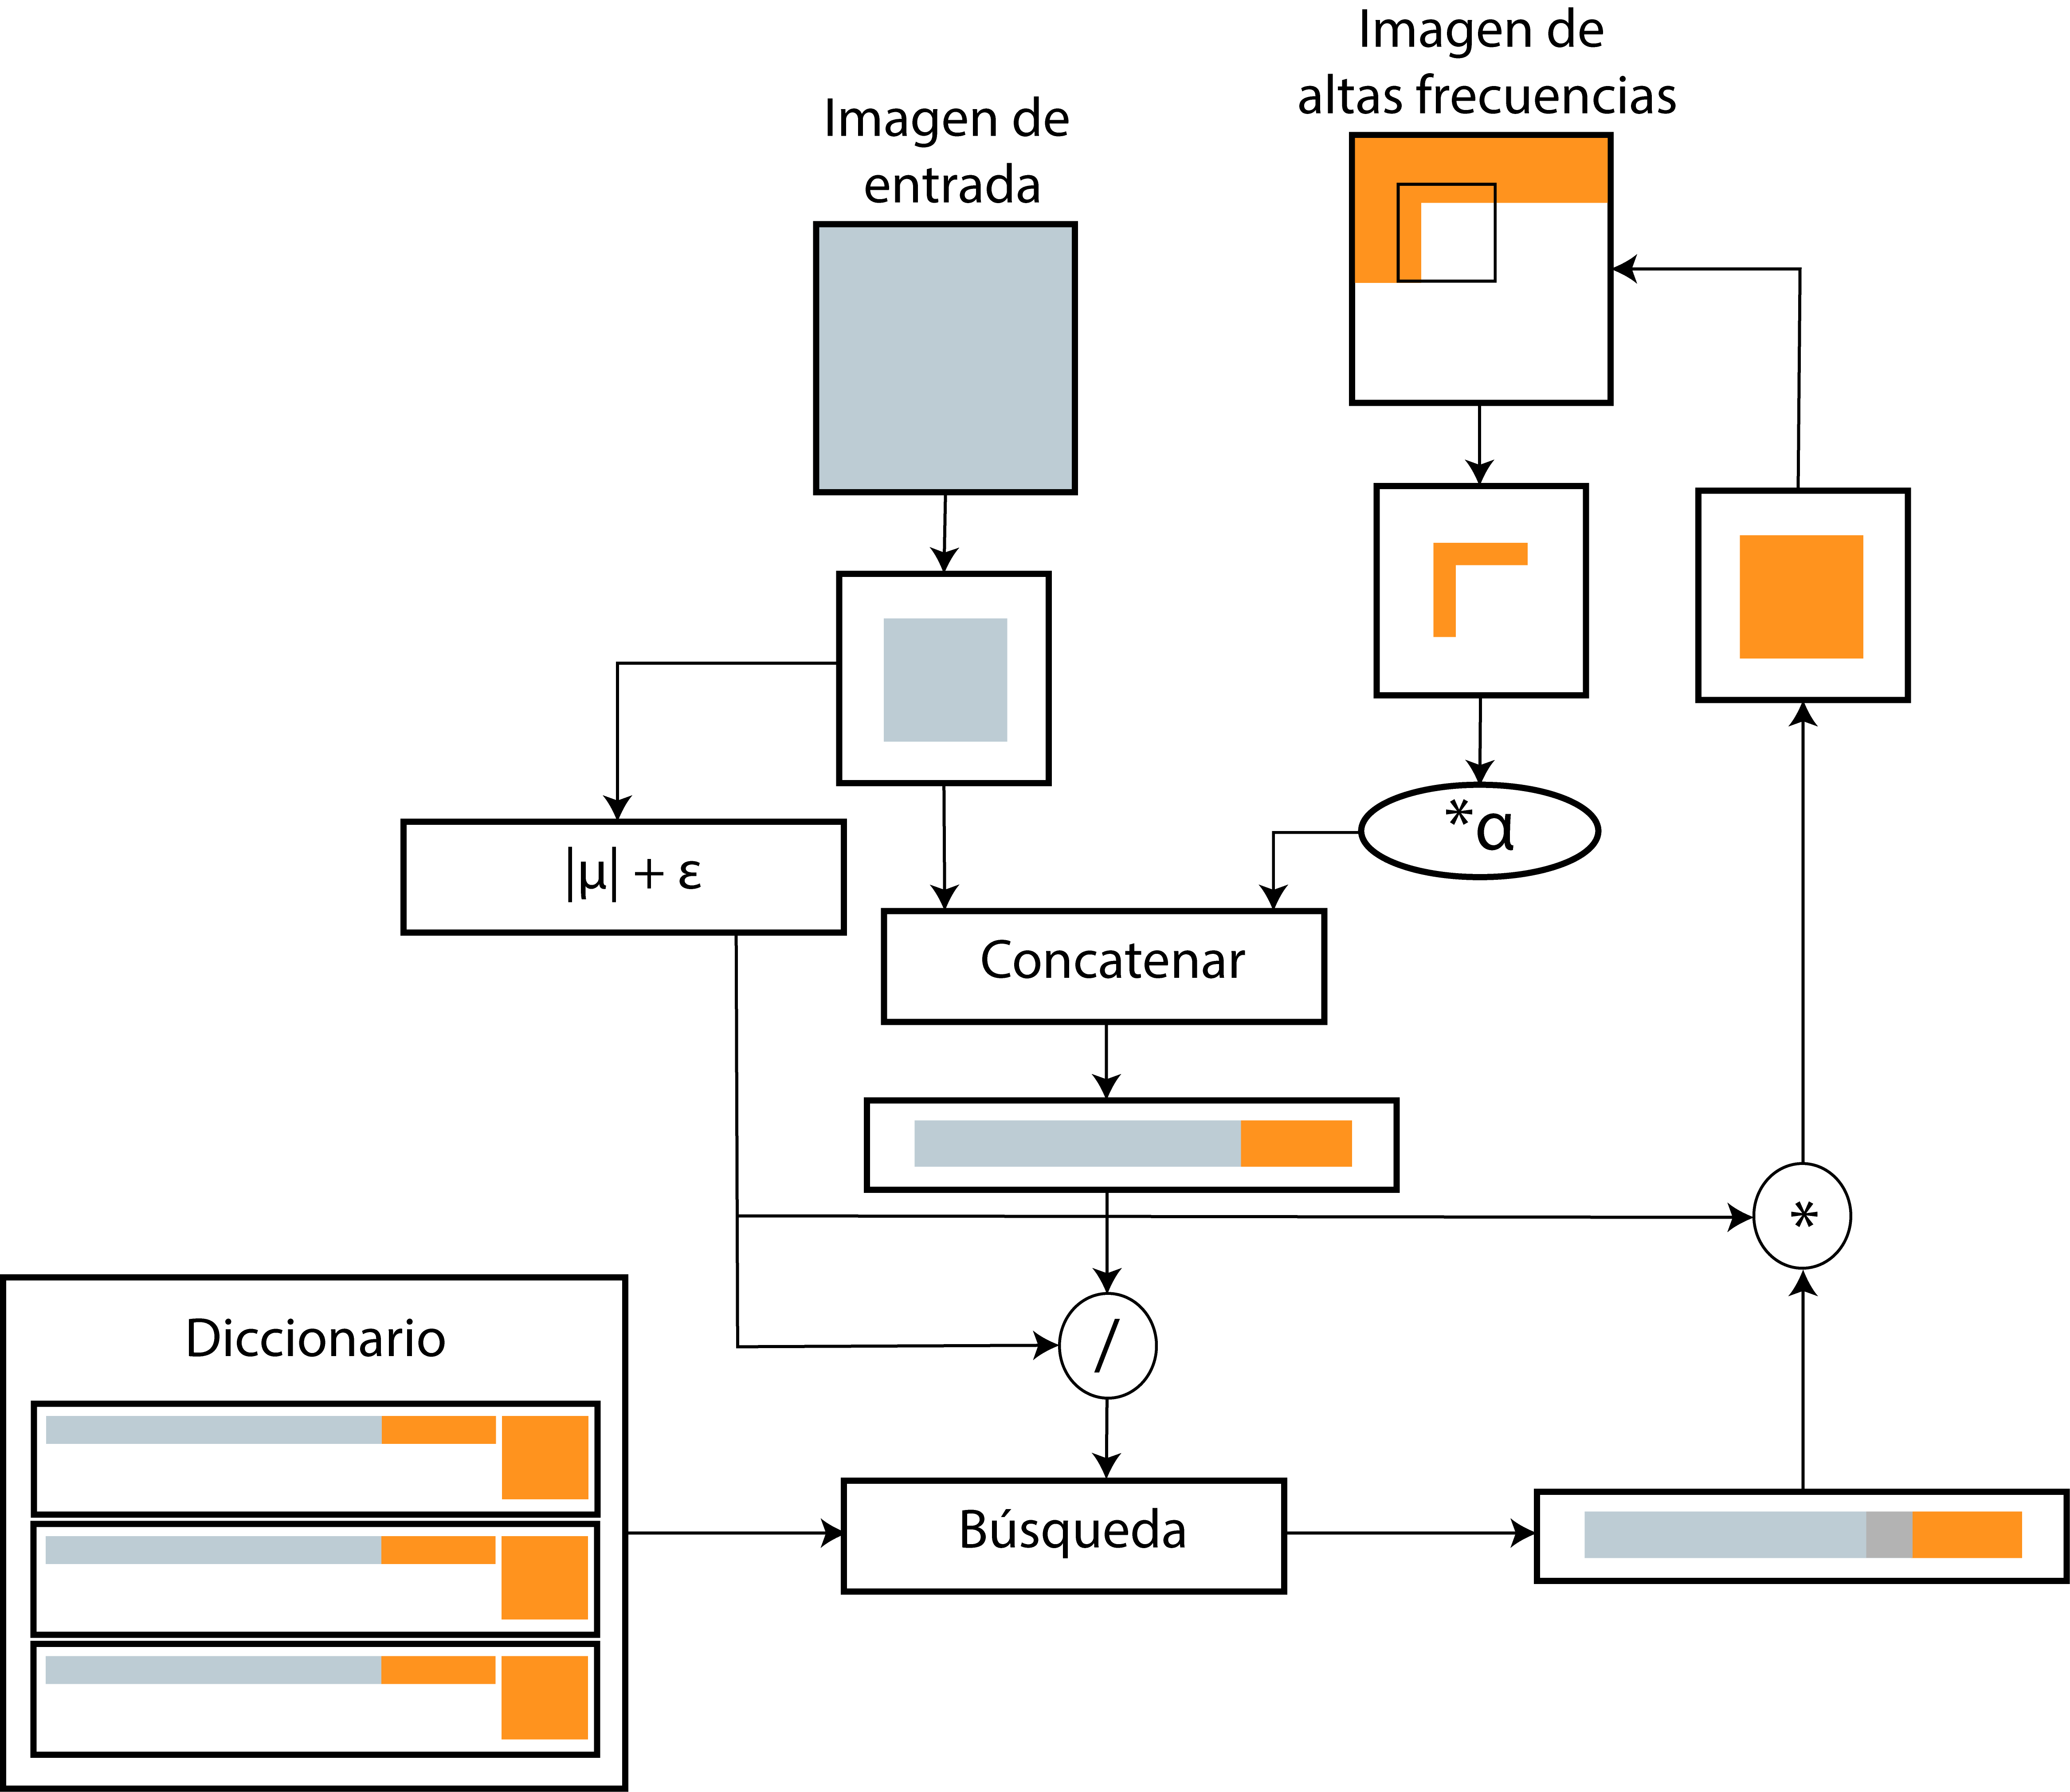
\includegraphics[scale = 0.3]{ freeman_prediccion.png}
        \centering
        \caption{ Algoritmo de predicción de imagen de frecuencias altas }
        \label{fig:fr_prediccion}
    \end{figure}

\end{frame}

    \begin{frame}{SCRNN}
    Apartado de SCRNN :)
\end{frame}
    \begin{frame}{SRGAN}
    

   El modelo SRGAN (Super Resolution Generative Adversarial Network) fue
   propuesto en 2016. La principal innovación de este modelo es su función de Pérdida Perceptual.

       
   \begin{figure}[H]
       \begin{center}
         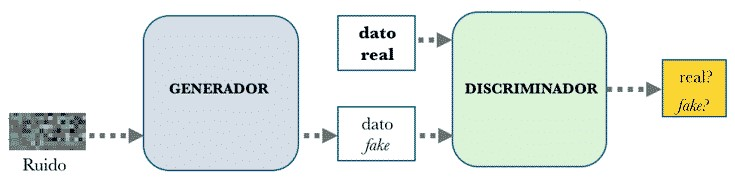
\includegraphics[scale = 0.5]{GANmodelo.jpg}
         \caption{Enfoques del Modelo Generador y Discriminador}
         \label{Alexis1}
       \end{center}
   \end{figure}
    

\end{frame}




\begin{frame}{SRGAN}

   \begin{block}{GAN}
      El termino \emph{Adversarial} se refiere a la dinámica 
      competitiva que se mantiene entre los dos modelos. Por un lado,
      el generador tiene por objetivo crear nuevos datos que sean indistinguibles del
      conjunto de entrenamiento, mientras que el discriminador debe poder ser capaz
      de distinguir cuáles son los datos creados y los reales.
   \end{block}
 
\end{frame}



\begin{frame}{Funcionamiento}
   \begin{figure}[H]
      \begin{center}
        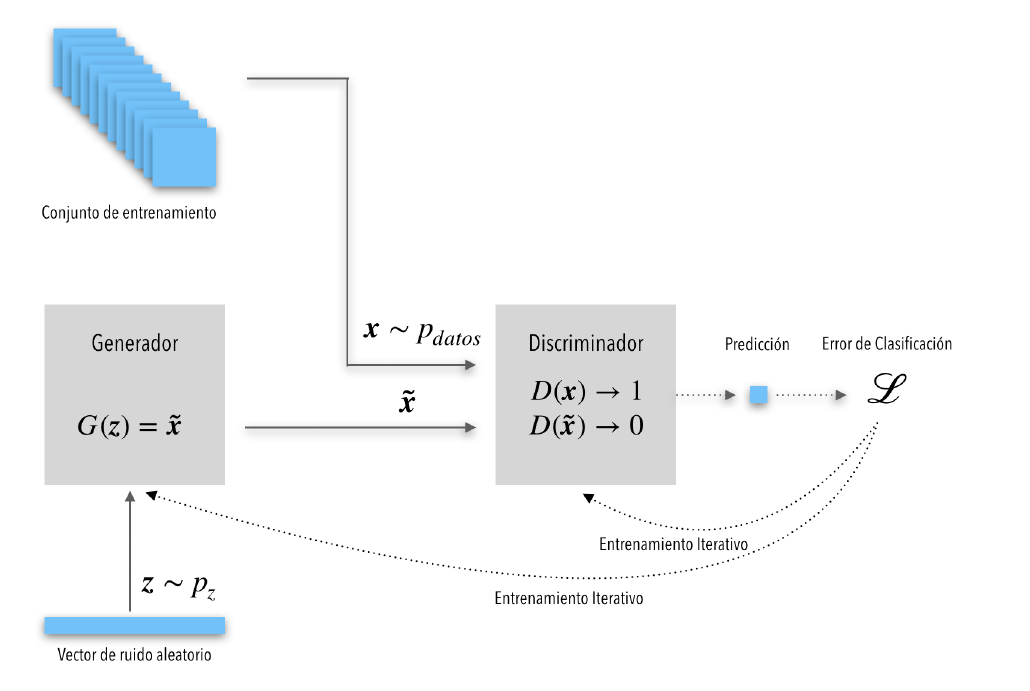
\includegraphics[scale = 0.5]{proceso_gan.png}
        \caption{Funciones del Modelo Generador y Discriminador}
        \label{Alexis2}
      \end{center}
   \end{figure}
   
\end{frame}

\begin{frame}{Desafios del modelo}
    
   \begin{block}{Principales fallas:}
       \begin{enumerate}
           \item  No convergencia:El generador y el discriminador no logran alcanzar un equilibrio.
           \item  Colapso modal:Esto ocurre cuando el generador produce muestras similares aunque las entradas sean de muy diversas características.
           \item  Pérdida no informativa: No es tan sencillo evaluar la mejora del modelo.
       \end{enumerate}
   \end{block}

\end{frame}

\begin{frame}{Funcionamiento}
   \begin{figure}[H]
      \begin{center}
        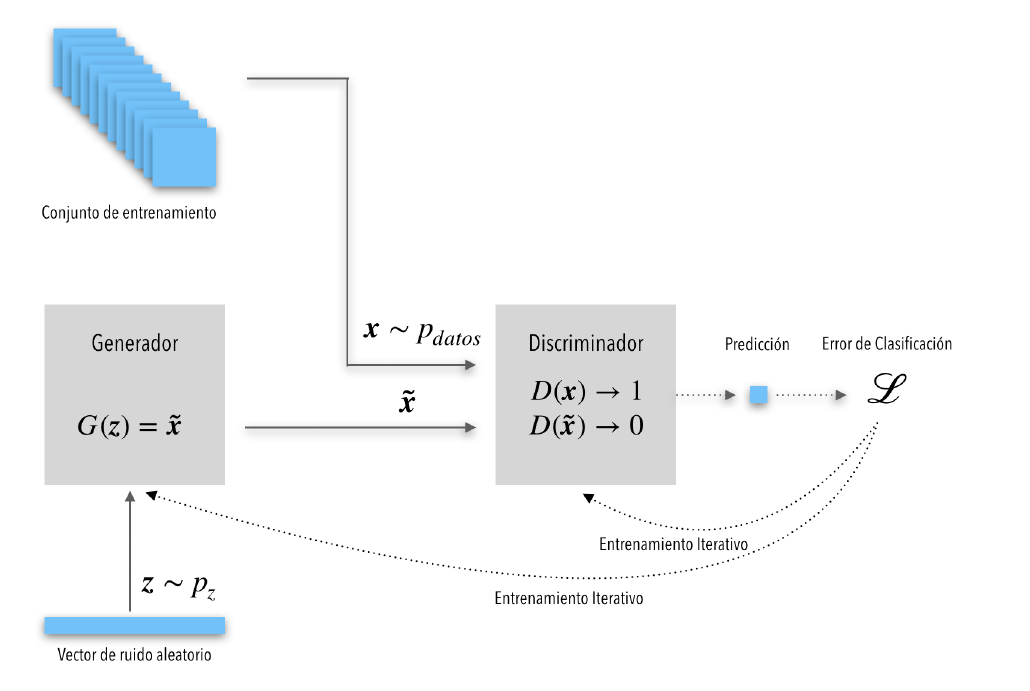
\includegraphics[scale = 0.5]{proceso_gan.png}
        \caption{Funciones del Modelo Generador y Discriminador}
        \label{Alexis9}
      \end{center}
   \end{figure}
   
\end{frame}

\section{Implementación}
    \begin{frame}{Freeman}
    Apartado de Freeman :)
\end{frame}
    \begin{frame}{SCRNN}
    Apartado de SCRNN :)
\end{frame}
    \begin{frame}{Modelo Discriminador}
    

    El modelo SRGAN (Super Resolution Generative Adversarial Network) fue
    propuesto en 2016 por un grupo de investigadores de la empresa Twitter.
    La principal innovación de este modelo es su función de pérdida, llamada
    función de pérdida perceptual, que permite mejorar el realismo de la imagen de
    salida.

        
    \begin{figure}[H]
        \begin{center}
          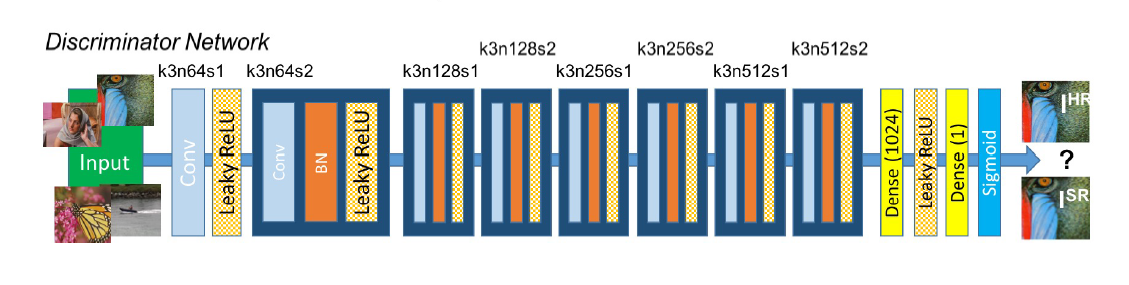
\includegraphics[scale = 0.5]{Imp_discriminador.png}
          \caption{Modelo de entrenamiento del discriminador}
          \label{Alexis3}
        \end{center}
    \end{figure}
     

\end{frame}

\begin{frame}{Modelo Generador}
    

    El modelo SRGAN (Super Resolution Generative Adversarial Network) fue
    propuesto en 2016 por un grupo de investigadores de la empresa Twitter.
    La principal innovación de este modelo es su función de pérdida, llamada
    función de pérdida perceptual, que permite mejorar el realismo de la imagen de
    salida.

        
    \begin{figure}[H]
        \begin{center}
          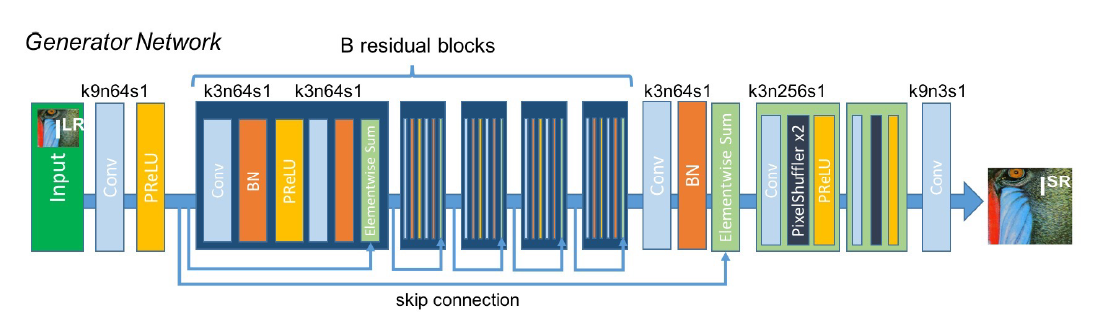
\includegraphics[scale = 0.5]{Imp_generador.png}
          \caption{Modelo de entrenamiento del generador}
          \label{Alexis4}
        \end{center}
    \end{figure}
     

\end{frame}



\begin{frame}{Redes residuales}
    \begin{block}{Bloque Residual}
        hacen la conexión entre capas anteriores con capas futuras (saltos) sin que la información de 
        las características extraídas en capas previas se diluya.
    \end{block}
    \begin{figure}[H]
        \begin{center}
          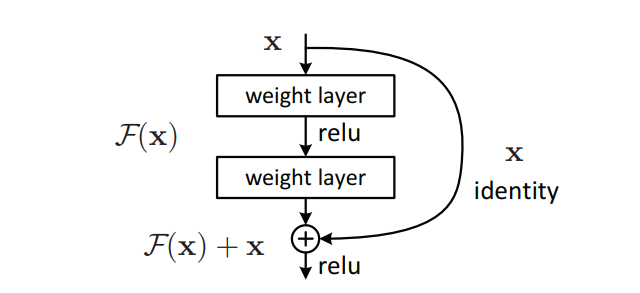
\includegraphics[scale = 0.4]{Residual-Block.png}
          \caption{Funcionamiento del Bloque Residual}
          \label{Alexis10}
        \end{center}
    \end{figure}

\end{frame}


\begin{frame}{Bloques de escalado}
    \begin{figure}[H]
        \begin{center}
          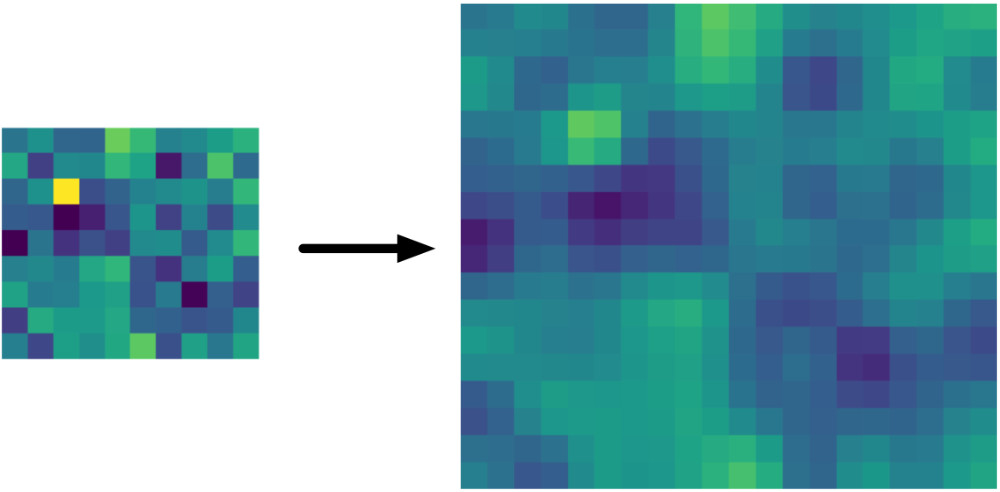
\includegraphics[scale = 0.4]{Bilinear2x.jpg}
          \caption{Red Neuronal Pre-entrenada}
          \label{Alexis5}
        \end{center}
    \end{figure}
     
\end{frame}

\begin{frame}{VGG19}
    
\begin{block}{Red Pre-entrenada}
    Se utiliza una red de entrenamiento pre-entrenada conocida como VGG19
    la cual nos da los pesos necesarios
\end{block}
    \begin{figure}[H]
        \begin{center}
          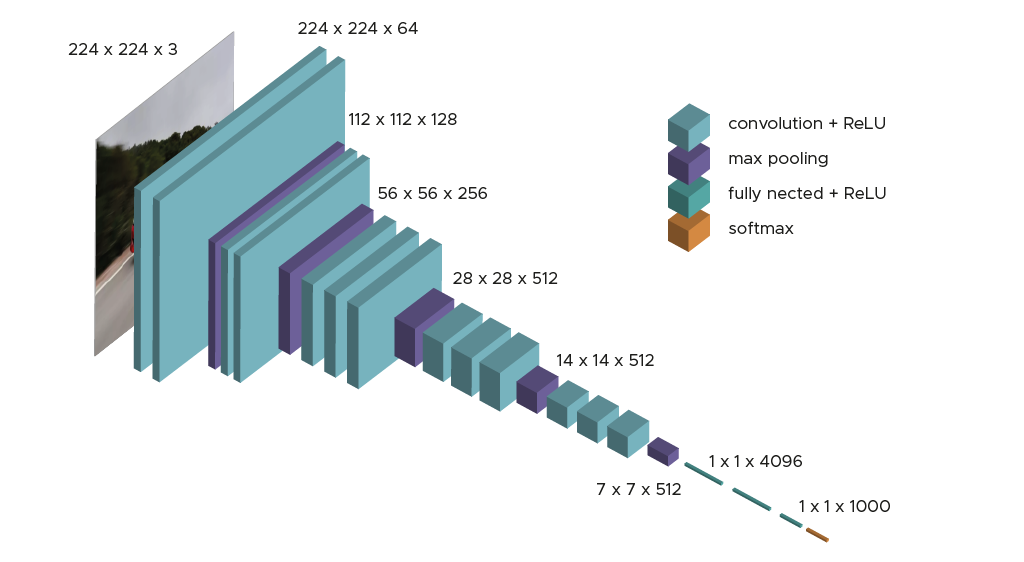
\includegraphics[scale = 0.18]{VGG19.png}
          \caption{Red Neuronal Pre-entrenada}
          \label{Alexis5}
        \end{center}
    \end{figure}
     

\end{frame}


\begin{frame}{Modelos Generadores obtenidos}
    
    \begin{figure}[H]
        \begin{center}
          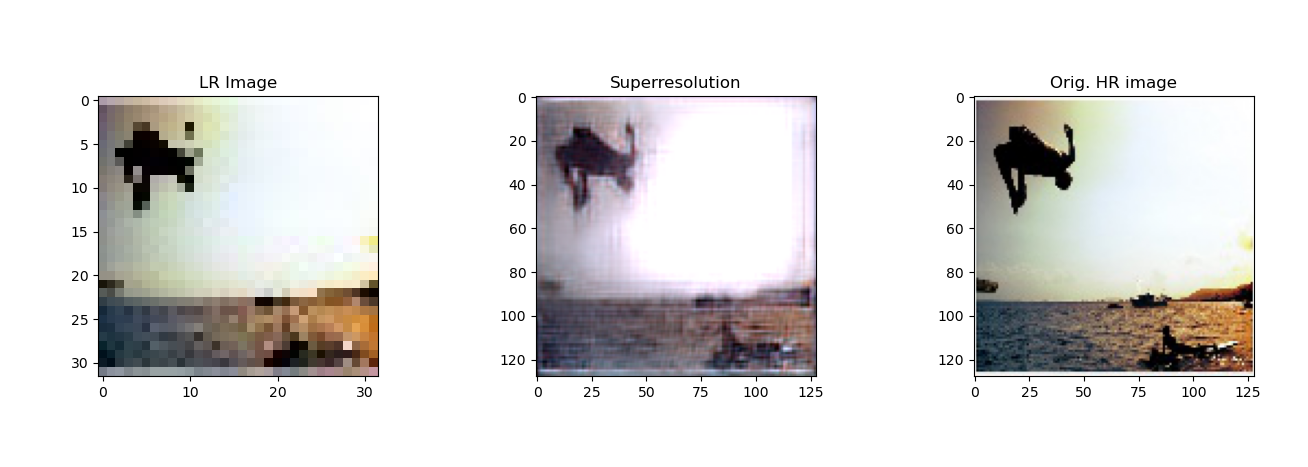
\includegraphics[scale = 0.6]{13im_200E.png}
          \caption{Modelo de entrenamiento del generador}
          \label{Alexis6}
        \end{center}
    \end{figure}
    
\end{frame}

\begin{frame}{Modelos Generadores obtenidos}
    
    \begin{figure}[H]
        \begin{center}
          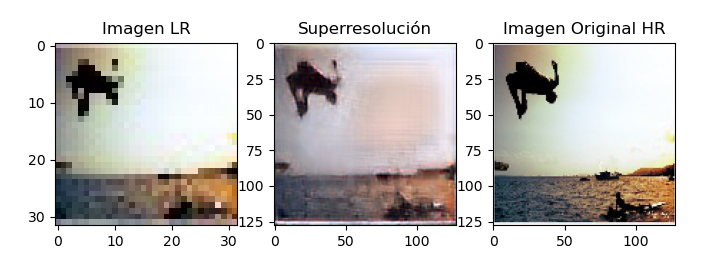
\includegraphics[scale = 0.6]{50im_400E.png}
          \caption{Modelo entrenado con 50 imágenes y 400 épocas}
          \label{Alexis7}
        \end{center}
    \end{figure}
     
\end{frame}


\begin{frame}{Modelos Generadores obtenidos}
    
    \begin{figure}[H]
        \begin{center}
          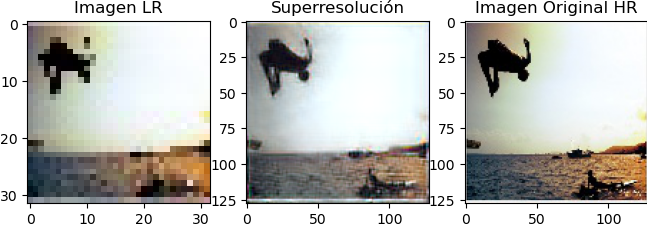
\includegraphics[scale = 0.5]{1000im_5E_Reentrenado.png}
          \caption{Modelo reentrenado 1000 imágenes, 5 épocas}
          \label{Alexis8}
        \end{center}
    \end{figure}
     
\end{frame}

\begin{frame}{Perdidas del modelo}
    
    \begin{figure}[H]
        \begin{center}
          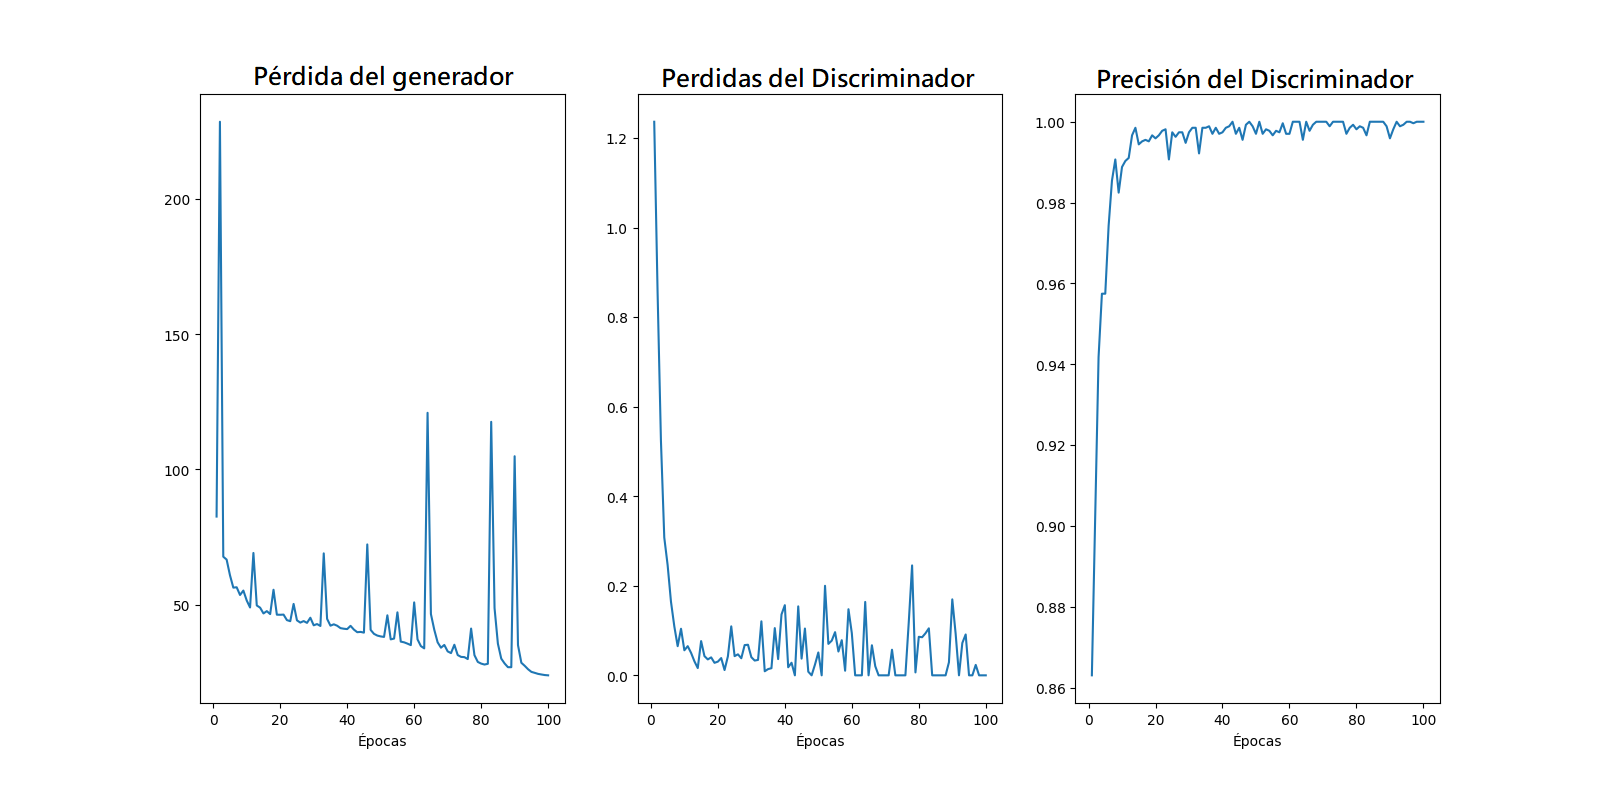
\includegraphics[scale = 0.5]{Graficasperdidas.png}
          \caption{Pérdidas y Precisión del Modelo}
          \label{Alexis8}
        \end{center}
    \end{figure}
     
\end{frame}


\section{Resultados}
    \begin{frame}{Resultados (1/3)}

    \begin{figure}[H]
        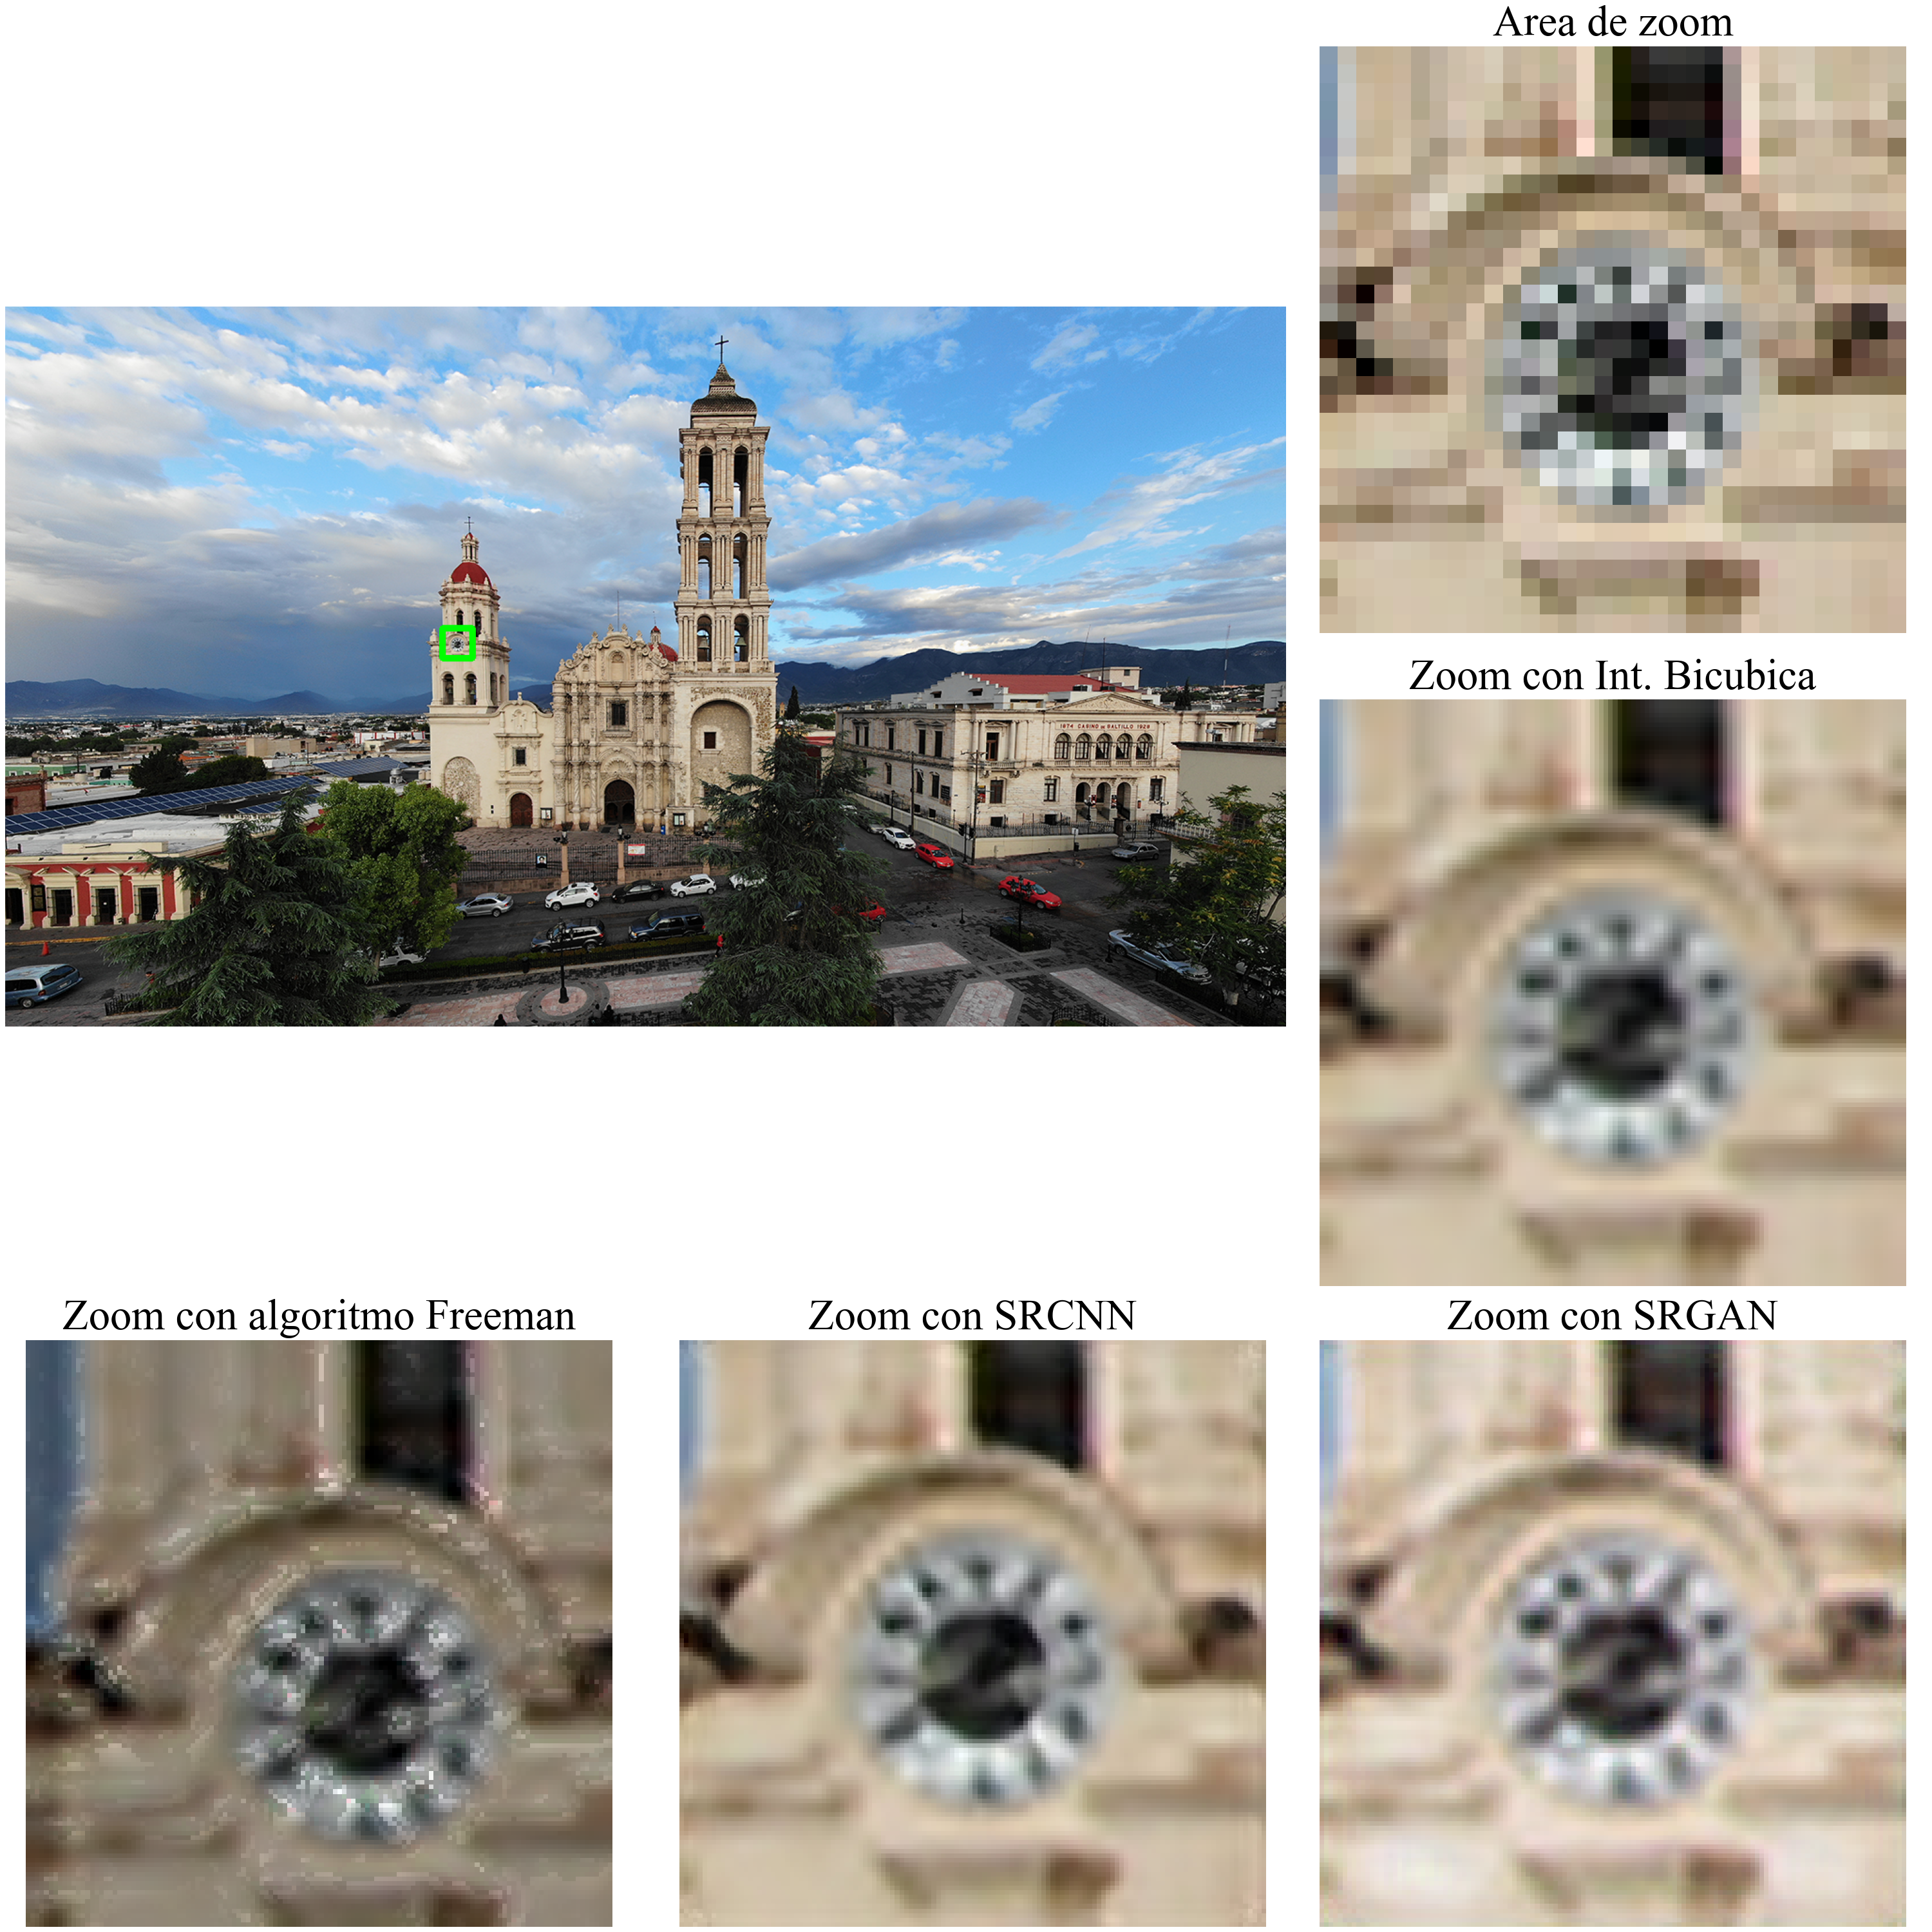
\includegraphics[scale = 0.16]{ ResultadoSaltillo.png}
        \centering
        \caption{Zoom digital en fotografía de Saltillo, Coahuila}
        \label{fig:saltillo}
    \end{figure}

\end{frame}

\begin{frame}{Resultados (2/3)}

    \begin{figure}[H]
        \includegraphics[scale = 0.16]{ ResultadoVilla.png}
        \centering
        \caption{Zoom digital en fotografía de Villahermosa, Tabasco}
        \label{fig:villahermosa}
    \end{figure}
    
\end{frame}

\begin{frame}{Resultados (3/3)}

    \begin{figure}[H]
        \includegraphics[scale = 0.16]{ ResultadoComitan.png}
        \centering
        \caption{Zoom digital en fotografía de Comitán, Chiapas}
        \label{fig:comitan}
    \end{figure}
    
\end{frame}

\section{Conclusiones}
    \begin{frame}{Conclusiones}
    \begin{block}{}
        \begin{itemize}
            \item La predicción de frecuencias altas resultó útil cuando se 
            requiere mejorar la resolución de una imagen.
            \pause
            \item \emph{SRCNN} y \emph{SRGAN} son más robustas y rápidas en la predicción 
            de la imagen para mejorar su resolución. 
            \pause
            \item El algoritmo de \emph{Freeman et al} tiene una muy buena aproximación
            y su 'entrenamiento' no es tan tardado como los métodos con redes neuronales. 
            \pause
            \item El comportamiento de los tres métodos fue el esperado y representan
            una evolución en tareas de \emph{Súper Resolución}. 
        \end{itemize}
    \end{block}
\end{frame}

\section{Código}
    \begin{frame}{Repositorio}
        En el siguiente enlace puede acceder al repositorio
        que contiene por carpetas la implementación de cada 
        método junto con su respectiva \emph{dataset}. 

        \vspace{1cm}
        \textbf{Repositorio: } \href{https://github.com/atevera/algoritmos-super-resolucion}{algoritmos-super-resolucion}

    \end{frame}

\section{Discusiones}
    \begin{frame}{Discusiones}
    Apartado de discusiones :)
\end{frame}

\section{Referencias}
    \begin{frame}{Referencias}
    \nocite{*}
    \bibliographystyle{plain}
    \bibliography{bibliografia}
\end{frame}

\end{document}